\begin{lemma}
    \label{lem:b_c_same_img_exist_a}
    Consider the pushout square in $\mathbf{Graph}$ of form
    \begin{center}{\normalfont
        \begin{tikzpicture}[node distance=12mm]
          \node (A) {$A$};
          \node [right of=A] (B) {$B$}; 
          \node [below of=A] (C) {$C$}; 
          \node [below of=B] (D) {$D$}; 
          \node () [at=($(A)!0.5!(D)$)] {\normalfont PO};
          \draw [>->] (A) to (B);
          \draw [>->] (A) to (C);
          \draw [>->] (B) to (D); 
          \draw [>->] (C) to (D);
        \end{tikzpicture}
    }\end{center} 
    The following hold 
    \begin{enumerate}
        \item  If $ b\in B $ and $ c \in C $ such that $ h_{BD}(b) = h_{CD}(c) $ then there is $ a \in A $ such that $ h_{AB}(a) = b $ and $ h_{AC}(a)= c $.
        \item  For all \( b \in B \setminus h_{AB}(A) \) and \( c \in C \), we have \( \beta'(b) \neq \alpha'(c) \).
    \end{enumerate}
\end{lemma}
\begin{proof}
     Let \( b \in B \) and \( c \in C \) such that \( h_{BD}(b) = h_{CD}(c) \). 
     
     There are two cases: if $b$ and $c$ are two nodes then let \( S \) be the singleton graph with a unique node \( u \), otherwise\textemdash$b$ and $c$ must be two edges with the same label $l$\textemdash let \( S \) be the graph with two distinct nodes and a unique edge \( u \) labeled by $l$.
     
     Define morphisms \( h_{SB}: S \to B \) and \( h_{SC}: S \to C \) such that \( h_{SB}(u) = b \) and \( h_{SC}(u) = c \). We have \( h_{SB} \star h_{BD} = h_{SC} \star h_{CD} \). The pushout square \( ACDB \) along monomorphisms is also a pullback square by~\autoref{prop:pb_eq_po}, and the universal property of the pullback guarantees the existence of a unique morphism \( h_{SA}: S \to A \) such that \( h_{SA} \star h_{AB} = h_{SB} \) and \( h_{SA} \star h_{AC} = h_{SC} \). Let \( a = h_{SA}(u) \). We have \( a \in A \), and by composition: 
     \begin{itemize}
        \item \(h_{AB}(a) = (h_{SA} \star h_{AB})(u) = h_{SB}(u) = b \)
        \item \(h_{AC}(a) = (h_{SA} \star h_{AC})(u) = h_{SC}(u) = c\)
     \end{itemize} 

    The second assertion is a direct consequentce of the first. Suppose, for contradiction, there exist \( b \in B \setminus h_{AB}(A) \) and \( c \in C \) such that \( h_{BD}(b) = h_{CD}(c) \). Since the first assertion holds, there must exist \( a \in A \) with \( h_{AB}(a) = b \) and \( h_{AC}(a) = c \). However, this contradicts the assumption that \( b \notin h_{AB}(A) \).
    \qed
\end{proof}

\begin{lemma}
    \label{kpcpck_pullback}
    Consider the following commutative diagram in \textbf{Graph}.
    \begin{center}
        \resizebox{6cm}{!}{
            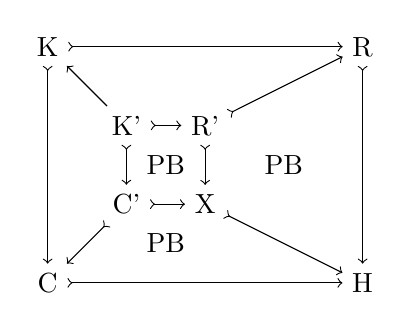
\begin{tikzpicture}
                \node (k) at (0,0) {K};
                \node (r) at (4,0) {R};
                \node (c) at (0,-3) {C};
                \node (h) at (4,-3) {H};
                \draw[<-<]  (r) -- (k) node [midway,above] {};
                \draw[>->] (c) -- (h) node [midway, below] {};
                \draw[>->] (r) -- (h) node[midway, left] {};
                \draw[>->] (k) -- (c) node[midway, left] {};
                \node (k') at (1,-1) {K'};
                \node (r') at (2,-1) {R'};
                \node (c') at (1,-2) {C'};
                \node () at (1.5,-1.5) {PB};
                \node () at (3,-1.5) {PB};
                \node () at (1.5,-2.5) {PB};
                \node (x) at (2,-2) {X};
                \draw [>->] (c') -- (x);
                \draw [>->] (r') -- (x);
                \draw [>->] (k') -- (r');
                \draw [>->] (k') -- (c');
                \draw [>->] (c') -- (c);
                \draw[>->] (r') -- (r);
                \draw[>->] (x) -- (h);
                \draw[->] (k') -- (k);
            \end{tikzpicture}
        }
        \end{center}  
        The squares $K'KCC'$ and $K'KRR'$ are pulllback square.
\end{lemma}
\begin{proof}
    Let $K \leftarrow A \rightarrow C'$ be a span such that 
    \begin{flalign}
        h_{AK} \star h_{KC} = h_{AC'} \star h_{C'C} \label{hakhkchacp}
    \end{flalign}
    We have the following commutative diagram 

    \begin{center}
        \resizebox{0.3\textwidth}{!}{
            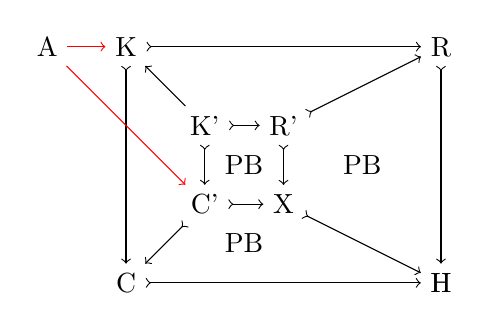
\begin{tikzpicture}
                \node (k) at (0,0) {K};
                \node (r) at (4,0) {R};
                \node (c) at (0,-3) {C};
                \node (h) at (4,-3) {H};
                \node (h) at (4,-3) {H};
                \node (a) at (-1,0) {A};
                \draw[<-<]  (r) -- (k) node [midway,above] {};
                \draw[>->] (c) -- (h) node [midway, below] {};
                \draw[>->] (r) -- (h) node[midway, left] {};
                \draw[>->] (k) -- (c) node[midway, left] {};
                \node (k') at (1,-1) {K'};
                \node (r') at (2,-1) {R'};
                \node (c') at (1,-2) {C'};
                \node () at (1.5,-1.5) {PB};
                \node () at (3,-1.5) {PB};
                \node () at (1.5,-2.5) {PB};
                \node (x) at (2,-2) {X};
                \draw [>->] (c') -- (x);
                \draw [>->] (r') -- (x);
                \draw [>->] (k') -- (r');
                \draw [>->] (k') -- (c');
                \draw [>->] (c') -- (c);
                \draw[>->] (r') -- (r);
                \draw[>->] (x) -- (h);
                \draw[->] (k') -- (k);
                \draw[->,red] (a) -- (c');
                \draw[->,red] (a) -- (k);
            \end{tikzpicture}
        }
        \end{center} 
    We show first the existence of a morphism $h_{AK'} \colon A \to K'$ such that 
    \begin{flalign*}
        h_{AK'} \star h_{K'C'} = h_{AC'}  
        \\
        h_{AK'} \star h_{K'K} = h_{AK} 
    \end{flalign*}
    From~\eqref{hakhkchacp}, we obtain 
    \begin{flalign}
        h_{AK} \star h_{KC} \star h_{CH}= h_{AC'} \star h_{C'C} \star h_{CH} \label{hakhkchchhacp}
    \end{flalign}
    From~\eqref{hakhkchchhacp} and commutativity of $C'CHX$ and $KCHR$, we have $h_{KC} \star h_{CH} = h_{KR} \star h_{RH}$ and $h_{C'C} \star h_{CH} = h_{C'X} \star h_{XH}$ and deduce  
     \begin{flalign}
        h_{AK} \star h_{KR} \star h_{RH}= h_{AC'} \star h_{C'X} \star h_{XH} \label{hakhkrhrhhacp}
     \end{flalign}
    Therefore, the following commutative diagram holds 

    \begin{center}
        \resizebox{0.3\textwidth}{!}{
            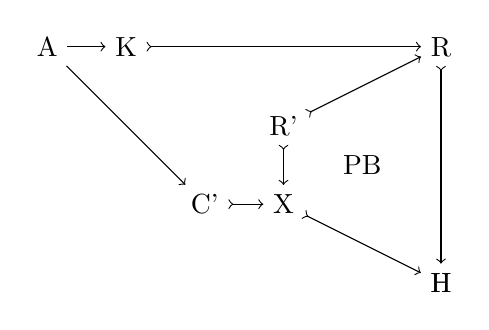
\begin{tikzpicture}
                \node (k) at (0,0) {K};
                \node (r) at (4,0) {R};
                \node (h) at (4,-3) {H};
                \node (h) at (4,-3) {H};
                \node (a) at (-1,0) {A};
                \draw[<-<]  (r) -- (k) node [midway,above] {};
                \draw[>->] (r) -- (h) node[midway, left] {};
                \node (r') at (2,-1) {R'};
                \node (c') at (1,-2) {C'};
                \node () at (3,-1.5) {PB};
                \node (x) at (2,-2) {X};
                \draw [>->] (c') -- (x);
                \draw [>->] (r') -- (x);
                \draw[>->] (r') -- (r);
                \draw[>->] (x) -- (h);
                \draw[->] (a) -- (c');
                \draw[->] (a) -- (k);
            \end{tikzpicture}
        }
        \end{center} 
    Since $R'XHR$ is a pullback square, by the universal property~\autoref{def:cat:pb}, there exists a unique morphism $h_{AR'} \colon A \to R'$ such that 
    \begin{flalign}
        h_{AR'} \star h_{R'R} = h_{AK} \star h_{KR}  \label{harprprakkr}
        \\
        h_{AR'} \star h_{R'X} = h_{AC'} \star h_{C'X} \label{harprpxacpcpx}
    \end{flalign}
    We have thus the following commutative diagram 

        \begin{center}
            \resizebox{0.2\textwidth}{!}{
                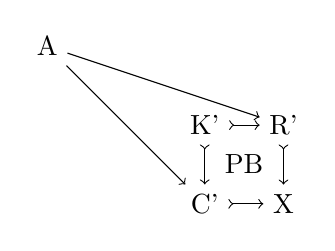
\begin{tikzpicture}
                    \node (a) at (-1,0) {A};
                    \node (k') at (1,-1) {K'};
                    \node (r') at (2,-1) {R'};
                    \node (c') at (1,-2) {C'};
                    \node () at (1.5,-1.5) {PB};
                    \node (x) at (2,-2) {X};
                    \draw [>->] (c') -- (x);
                    \draw [>->] (r') -- (x);
                    \draw [>->] (k') -- (r');
                    \draw [>->] (k') -- (c');
                    \draw[->] (a) -- (c');
                    \draw[->] (a) -- (r');
                \end{tikzpicture}
            }
        \end{center} 
    Since $K'C'XR'$ is a pullback square, there exists a unique morphism $h_{AK'} \colon A \to K'$ such that 
    \begin{flalign}
        h_{AK'} \star h_{K'C'} = h_{AC'}  \label{hakphkpcphacp}
        \\
        h_{AK'} \star h_{K'R'} = h_{AR'} \label{hakpkprparp}
    \end{flalign}
    We have $h_{AK'} \star h_{K'C'} = h_{AC'}$ by~\eqref{hakphkpcphacp}, and $h_{AK'} \star h_{K'K} = h_{AK}$ because $h_{KR}$ is injective and the following holds:
    \begin{flalign*}
        (h_{AK'} \star h_{K'K}) \star h_{KR} &= h_{AK} \star h_{K'R'} \star h_{R'R} \hspace{0.5cm} &\text{by commutativity of $K'KRR'$}\\
        &= h_{AR'} \star h_{R'R} &\text{by~\eqref{hakpkprparp}} \\
        &= h_{AK} \star h_{KR} &\text{by~\eqref{harprprakkr}}
    \end{flalign*}
    Now, we show the unicity of such a morphism from $A$ to $K'$. 
    Let $h_{AK'}' \colon A \to K'$ be a morphism  such that 
    \begin{flalign*}
        h_{AK'}' \star h_{K'C'} = h_{AC'}  
        \\
        h_{AK'}' \star h_{K'K} = h_{AK} 
    \end{flalign*}
    From $h_{AK'} \star h_{K'C'} = h_{AC'}$, $h_{AK'}' \star h_{K'C'} = h_{AC'}$ and injectivity of $h_{K'C'}$, we deduce $h_{AK'} = h_{AK'}$.

    \qed
\end{proof}


\begin{lemma}
    \label{kpcpxrp_po}
    Consider the following commutative diagram in \textbf{Graph} where $KCHR$ is a pushout.
    \begin{center}
        \resizebox{6cm}{!}{
            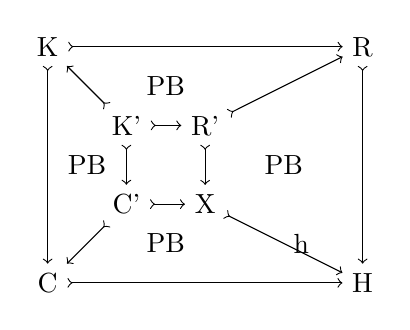
\begin{tikzpicture}
                \node (k) at (0,0) {K};
                \node (r) at (4,0) {R};
                \node (c) at (0,-3) {C};
                \node (h) at (4,-3) {H};
                % \node (rb) at ($\scl*(1.5,-0.5)$) {$R_X$};
                % \node (h') at ($\scl*(1.5,-1.5)$) {$H'$};
                % \draw[>->]  (rb) -- (h') node [midway,above] {};
                % \draw[>->]  (c) -- (h') node [midway,above] {};
                \draw[<-<]  (r) -- (k) node [midway,above] {};
                \draw[>->] (c) -- (h) node [midway, below] {};
                \draw[>->] (r) -- (h) node[midway, left] {};
                \draw[>->] (k) -- (c) node[midway, left] {};
                % \draw[->] (rb) to (l);
                % \draw[<-<] (rb) to (k);
                \node (k') at (1,-1) {K'};
                \node (r') at (2,-1) {R'};
                \node (c') at (1,-2) {C'};
                % \node () at (1.5,-1.5) {PB};
                \node () at (3,-1.5) {PB};
                \node () at (1.5,-2.5) {PB};
                \node () at (1.5,-0.5) {PB};
                \node () at (0.5,-1.5) {PB};
                \node (x) at (2,-2) {X};
                % \draw [->] (x) -- (h') node[midway] {!};
                \draw [>->] (c') -- (x);
                \draw [>->] (r') -- (x);
                \draw [>->] (k') -- (r');
                \draw [>->] (k') -- (c');
                \draw [>->] (c') -- (c);
                % \draw [->] (r') -- (rb);
                % \draw [->] (r') -- (rb);
                % \draw [->] (h') -- (h);
                \draw[>->] (r') -- (r);
                \draw[>->] (x) -- (h) node[midway,right] {h};
                % \node (rb) at ($\scl*(\sclx*1.5,-0.5)$) {$R_X$};
                % \node (h') at ($\scl*(\sclx*1.5,-1.2)$) {$H'$};
                % \draw[>->]  (rb) -- (h') node [midway,above] {};
                % \draw[>->]  (c) -- (h') node [midway,above] {};
                % \draw[>->]  (rb) -- (h') node [midway,above] {};
                % \draw[>->] (rb) to (r);
                % \draw[<-<] (rb) to (k);
                \draw[>->] (k') -- (k) ;
            \end{tikzpicture}
        }
        \end{center} 
        The square $K'C'XR'$ is a pushout.
\end{lemma}
\begin{proof}
    \textbf{Graph} is adhesive by~\autoref{prop:graph_adhesive}. By~\autoref{def:adhesive_cat}, pushouts along monomorphisms are VK squares in \textbf{Graph}. The square $KCHR$ is a pushout along monomorphisms in \textbf{Graph}. Hence $KCHR$ is VK square. By~\autoref{def:vk_square}, the square $K'C'XR'$ is pushout if the squares $C'CHX$ and $R'XHR$ are pullbacks. By assumption, the squares $C'CHX$ and $R'XHR$ are pullbacks. Therefore, $K'C'XR'$ is pushout.
\end{proof} 

\begin{lemma}
    \label{lem:xinXcpinCrpinR}
        Consider the following pushout square in \textbf{Graph}.
    \begin{center}
        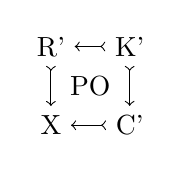
\begin{tikzpicture}
            \node (k') at (-1,-1) {K'};
            \node (r') at (-2,-1) {R'};
            \node (c') at (-1,-2) {C'};
            \node (x) at (-2,-2) {X};
            \node () at (-1.5,-1.5) {PO};
            \draw [>->] (c') -- (x);
            \draw [>->] (r') -- (x);
            \draw [>->] (k') -- (r');
            \draw [>->] (k') -- (c');
        \end{tikzpicture}
    \end{center}
     Let $x$ be a node (resp. an edge) in $X$. There is either a node (resp. an edge) $r'$ in $R'$ such that $h_{R'X}(r') = x$ or a node (resp. an edge) $c'$ in $C'$ such that $h_{C'X}(c') = x$.
\end{lemma}
\begin{proof}
    Suppose, by contradiction, that there exists neither a node (resp. an edge) $r'$ in $R'$ such that $h_{R'X}(r') = x$ nor a node (resp. an edge) $c'$ in $C'$ such that $h_{C'X}(c') = x$.

    Let $G$ be a graph with two distinct nodes (resp. edges) $y$ and $y'$.
    By the universal property of pushout square~\autoref{def:cat:po}, there exists a unique morphism $h_{XG}:X \rightarrowtail G$ such that $h_{C'G} = h_{C'X} \star h_{XG}$ and  $h_{R'G} = h_{R'X} \star h_{XG}$.
    \begin{center}
        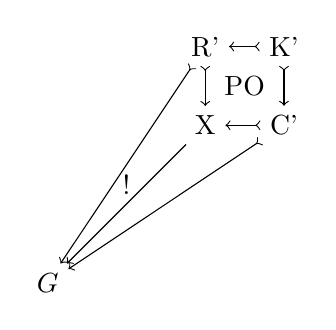
\begin{tikzpicture}
            \node (g) at (-4,-4) {$G$};
            \node (k') at (-1,-1) {K'};
            \node (r') at (-2,-1) {R'};
            \node (c') at (-1,-2) {C'};
            \node (x) at (-2,-2) {X};
            \node () at (-1.5,-1.5) {PO};
            \draw [>->] (c') -- (x);
            \draw [>->] (r') -- (x);
            \draw [>->] (k') -- (r');
            \draw [>->] (k') -- (c');
            \draw [>->] (c') -- (g);
            \draw [>->] (r') -- (g);
            \draw [->] (x) -- (g) node[midway,above] {!};
        \end{tikzpicture}
    \end{center}
    However, if we define two morphisms $f$ and $g$ by 
    \begin{flalign*}
        f(z) &= h_{XG}(z) \text{if $z \neq x$}\\
        f(x) &= y \\
        g(z) &= h_{XG}(z) \text{if $z \neq x$}\\
        g(x) &= y' \\
    \end{flalign*}
    we have $f \neq g$ and 
    \begin{flalign*}
        h_{C'G} = h_{C'X} \star f\\
        h_{R'G} = h_{R'X} \star f\\
        h_{C'G} = h_{C'X} \star g\\
        h_{R'G} = h_{R'X} \star g
    \end{flalign*}
    which is a contradiction.
\end{proof}

\begin{lemma}
    \label{lem:g_monic}
    Consider the following commutative diagram in \textbf{Graph}.
    \begin{center}
        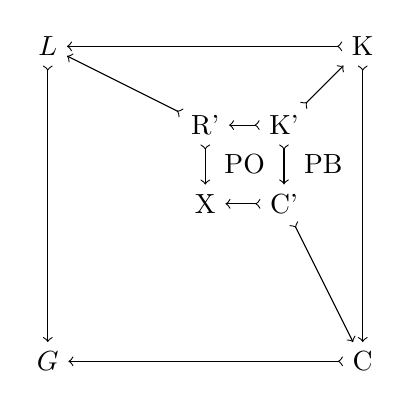
\begin{tikzpicture}
            \node (k) at (0,0) {K};
            \node (c) at (0,-4) {C};
            \node (l) at (-4,0) {$L$};
            \node (g) at (-4,-4) {$G$};
            \draw[>->] (l) -- (g) node [midway,above] {};
            \draw[>->] (c) -- (g) node [midway,above] {};
            \draw[>->] (k) -- (c) node[midway, left] {};
            \draw[<-<] (l) to (k);
            \node (k') at (-1,-1) {K'};
            \node (r') at (-2,-1) {R'};
            \node (c') at (-1,-2) {C'};
            \node (x) at (-2,-2) {X};
            \node () at (-1.5,-1.5) {PO};
            \node () at (-0.5,-1.5) {PB};
            \draw [>->] (c') -- (x);
            \draw [>->] (r') -- (x);
            \draw [>->] (k') -- (r');
            \draw [>->] (k') -- (c');
            \draw [>->] (c') -- (c);
            \draw [>->] (r') -- (l);
            \draw [>->] (k') -- (k);
        \end{tikzpicture}
    \end{center}
    There exists a unique monomorphism $h_{XG}:X \rightarrowtail G$ such that
    $C'XGC$ and $R'XGL$ are commutative squares.
    %  $h_{C'C} \star h_{CG} = h_{C'X} \star h_{XG}$ and  $h_{R'L} \star h_{LG} = h_{R'X} \star h_{XG}$.
\end{lemma}
\begin{proof}
    There exists a unique morphism $h_{XG}:X \to G$, by~\autoref{def:cat:po}, because $K'C'XR'$ is a pushout\todo{$K'C'XR'$ PO} and 
    $h_{K'C'} \star h_{C'C} \star h_{CG}
    =h_{K'R'} \star h_{R'L} \star h_{LG}$.
    % the following hold
    % \begin{flalign*}
    %     &h_{K'C'} \star h_{C'C} \star h_{CG} &\\ 
    %    =&h_{K'K} \star h_{KC} \star h_{CG} &\hspace{2cm}\text{by commutativity of $K'C'CK$}\\
    %    =&h_{K'K} \star h_{KL} \star h_{LG} &\text{by the commutativity of $KCGL$} \\
    %    =&h_{K'R'} \star h_{R'L} \star h_{LG} &\text{by the commutativity of $K'KLR'$}
    % \end{flalign*}
    Therefore, the following commutative diagram holds
    \begin{center}
        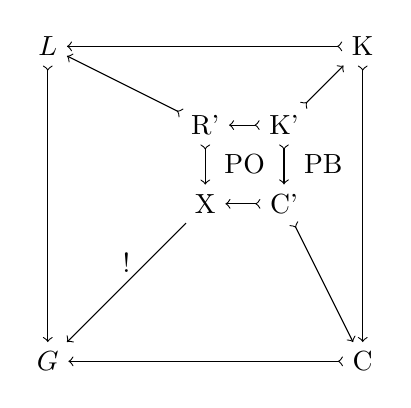
\begin{tikzpicture}
            \node (k) at (0,0) {K};
            \node (c) at (0,-4) {C};
            \node (l) at (-4,0) {$L$};
            \node (g) at (-4,-4) {$G$};
            \draw[>->] (l) -- (g) node [midway,above] {};
            \draw[>->] (c) -- (g) node [midway,above] {};
            \draw[>->] (k) -- (c) node[midway, left] {};
            \draw[<-<] (l) to (k);
            \node (k') at (-1,-1) {K'};
            \node (r') at (-2,-1) {R'};
            \node (c') at (-1,-2) {C'};
            \node (x) at (-2,-2) {X};
            \node () at (-1.5,-1.5) {PO};
            \node () at (-0.5,-1.5) {PB};
            \draw [>->] (c') -- (x);
            \draw [>->] (r') -- (x);
            \draw [>->] (k') -- (r');
            \draw [>->] (k') -- (c');
            \draw [>->] (c') -- (c);
            \draw [>->] (r') -- (l);
            \draw [>->] (k') -- (k);
            \draw [->] (x) -- (g) node[midway,above] {!};
        \end{tikzpicture}
    \end{center}
    It remains to show that $h_{XG}$ is injective.
    
    Let $x_1,x_2$ be two elements in the graph $X$ such that $x_1 \neq x_2$. Since $K'R'XC'$ is a pushout\todo{$K'R'XC'$ P.O.} square, by~\autoref{lem:xinXcpinCrpinR}, there are 4 possible cases:
    \begin{enumerate}
        \item there are $c_1, c_2 \in C'$ such that $h_{C'X}(c_1) = x_1$ and $h_{C'X}(c_2) = x_2$;
        \item there are $r_1, r_2 \in R'$ such that $h_{R'X}(r_1) = x_1$ and $h_{R'X}(r_2) = x_2$;
        \item there are $r' \in R'$ and $c' \in C'$ such that $h_{C'X}(c') = x_1$ and $h_{R'X}(r') = x_2$;
        \item there are $r' \in R'$ and $c' \in C'$ such that $h_{C'X}(c') = x_2$ and $h_{R'X}(r') = x_1$;
    \end{enumerate}
    Since the second and fourth cases are symmetric to the first and third case, respectively, it suffices to show that in the first and third cases, we have $h_{XG}(x_1) \neq h_{XG}(x_2)$. 
    \begin{itemize}
        \item[Case (1)] Suppose that there are $c_1, c_2 \in C'$ such that $h_{C'X}(c_1) = x_1$ and $h_{C'X}(c_2) = x_2$. 
        
        We have $c_1 \neq c_2$ since $x_1 \neq x_2$ and $h_{C'X}$ is injective.
        
        Therefore we have 
        \begin{flalign*}
            h_{XG}(x_1)&= h_{XG}(h_{C'X}(c_1)) & \text{by definition of $c_1$}\\
                        &= (h_{C'X} \star h_{XG})(c_1)  \\
                        &= (h_{C'C} \star h_{CG})(c_1) & \text{by commutativity of $C'CGX$} \\
                        &\neq (h_{C'C} \star h_{CG})(c_2) & \text{by injectivity of $h_{C'C} \star h_{CG}$ and $c_1 \neq c_2$} \\
                        &= (h_{C'X} \star h_{XG})(c_2) & \text{by commutativity of $C'CGX$} \\
                        &= h_{XG}(h_{C'X}(c_2)) \\
                        &= h_{XG}(x_2) & \text{by definition of $c_2$}
        \end{flalign*}
        
        % \begin{center}
        %     \begin{tikzpicture}
        %         \node (k) at (0,0) {K};
        %         \node (c) at (0,-4) {C};
        %         \node (l) at (-4,0) {$L$};
        %         \node (g) at (-4,-4) {$G$};
        %         \draw[>->] (l) -- (g) node [midway,above] {};
        %         \draw[>->] (c) -- (g) node [midway,above] {};
        %         \draw[>->] (k) -- (c) node[midway, left] {};
        %         \draw[<-<] (l) to (k);
        %         \node (k') at (-1,-1) {K'};
        %         \node (r') at (-2,-1) {R'};
        %         \node (c') at (-1,-2) {C'};
        %         \node (x) at (-2,-2) {X};
        %         \node () at (-1.5,-1.5) {PO};
        %         \node () at (-0.5,-1.5) {PB};
        %         \draw [>->] (c') -- (x);
        %         \draw [>->] (r') -- (x);
        %         \draw [>->] (k') -- (r');
        %         \draw [>->] (k') -- (c');
        %         \draw [>->] (c') -- (c);
        %         \draw [>->] (r') -- (l);
        %         \draw [>->] (k') -- (k);
        %         \draw [->] (x) -- (g) node[midway,above] {!};
        %     \end{tikzpicture}
        % \end{center}
        % \item[(2)] Suppose that there are $r_1, r_2 \in R'$ such that $h_{R'X}(r_1) = x_1$ and $h_{R'X}(r_2) = x_2$. The proof of this case is analogous to the previous case.

        % We have $r_1 \neq r_2$ because $x_1 \neq x_2$ and $h_{R'X}$ is injective, and
        % \begin{flalign*}
        %     h_{XG}(x_1) &= h_{XG}(h_{R'X}(r_1)) & \text{by definition of $r_1$}\\
        %                  &= (h_{R'X} \star h_{XG})(r_1)  \\
        %                  &= (h_{R'L} \star h_{LG})(r_1) & \text{by commutativity of $R'XGL$} \\
        %                  &\neq (h_{R'L} \star h_{LG})(r_2) & \text{by injectivity of $h_{R'L} \star h_{LG}$ and $r_1 \neq r_2$} \\
        %                  &= (h_{R'X} \star h_{XG})(r_2) & \text{by commutativity of $R'XGL$} \\
        %                  &= h_{XG}(h_{R'X}(r_2)) \\
        %                  &= h_{XG}(x_2) & \text{by definition of $r_2$}
        % \end{flalign*}
        
        % \begin{center}
        %     \begin{tikzpicture}
        %         \node (k) at (0,0) {K};
        %         \node (c) at (0,-4) {C};
        %         \node (l) at (-4,0) {$L$};
        %         \node (g) at (-4,-4) {$G$};
        %         \draw[>->] (l) -- (g) node [midway,above] {};
        %         \draw[>->] (c) -- (g) node [midway,above] {};
        %         \draw[>->] (k) -- (c) node[midway, left] {};
        %         \draw[<-<] (l) to (k);
        %         \node (k') at (-1,-1) {K'};
        %         \node (r') at (-2,-1) {R'};
        %         \node (c') at (-1,-2) {C'};
        %         \node (x) at (-2,-2) {X};
        %         \node () at (-1.5,-1.5) {PO};
        %         \node () at (-0.5,-1.5) {PB};
        %         \draw [>->] (c') -- (x);
        %         \draw [>->] (r') -- (x);
        %         \draw [>->] (k') -- (r');
        %         \draw [>->] (k') -- (c');
        %         \draw [>->] (c') -- (c);
        %         \draw [>->] (r') -- (l);
        %         \draw [>->] (k') -- (k);
        %         \draw [->] (x) -- (g) node[midway,above] {!};
        %     \end{tikzpicture}
        % \end{center}
        \item[Case (3)] Suppose that there are $r' \in R'$ and $c' \in C'$ such that $h_{C'X}(c') = x_1$ and $h_{R'X}(r') = x_2$.
        % , or $h_{C'X}(c') = x_2$ and $h_{R'X}(r') = x_1$. By symmetry, we suppose that the first case holds. Let $c = h_{C'C}(c')$ and $l = h_{R'L}(r')$
        
        We have three cases:
            \begin{itemize}
                \item[(3.1)] Suppose that $h_{C'C}(c') \notin \operatorname{Im}(h_{KC})$. We have
                    \begin{flalign*}
                        h_{XG}(x_1) &= h_{XG}(h_{C'X}(c')) & \text{by definition of $c'$}\\
                                     &= (h_{C'X} \star h_{XG})(c') \\
                                     &= (h_{C'C} \star h_{CG})(c') & \text{by commutativity of $C'CGX$} \\
                                     &= h_{CG}(h_{C'C}(c')) & \\
                                    %  &= h_{CG}(c) & \\
                                     &\neq 
                                    %  h_{LG}(l) & \text{by~\autoref{lem:b_c_same_img_exist_a} and $c\notin \operatorname{Im}(h_{KC})$}  
                                    h_{LG}(h_{R'L}(r')) & \text{by~\autoref{lem:b_c_same_img_exist_a} and $h_{C'C}(c') \notin \operatorname{Im}(h_{KC})$}   
                                    \\
                                     &= (h_{R'L} \star h_{LG})(r') 
                                     \\
                                     &= (h_{R'X} \star h_{XG})(r') & \text{by commutativity of $R'XGL$} 
                                     \\
                                     &= h_{XG}(h_{R'X}(r'))
                                     \\
                                     &= h_{XG}(x_2) & \text{by definition of $r'$}
                    \end{flalign*}
                    
                    % \begin{center}
                    %     \begin{tikzpicture}
                    %         \node (k) at (0,0) {K};
                    %         \node (c) at (0,-4) {C};
                    %         \node (l) at (-4,0) {$L$};
                    %         \node (g) at (-4,-4) {$G$};
                    %         \draw[>->] (l) -- (g) node [midway,above] {};
                    %         \draw[>->] (c) -- (g) node [midway,above] {};
                    %         \draw[>->] (k) -- (c) node[midway, left] {};
                    %         \draw[<-<] (l) to (k);
                    %         \node (k') at (-1,-1) {K'};
                    %         \node (r') at (-2,-1) {R'};
                    %         \node (c') at (-1,-2) {C'};
                    %         \node (x) at (-2,-2) {X};
                    %         \node () at (-1.5,-1.5) {PO};
                    %         \node () at (-0.5,-1.5) {PB};
                    %         \draw [>->] (c') -- (x);
                    %         \draw [>->] (r') -- (x);
                    %         \draw [>->] (k') -- (r');
                    %         \draw [>->] (k') -- (c');
                    %         \draw [>->] (c') -- (c);
                    %         \draw [>->] (r') -- (l);
                    %         \draw [>->] (k') -- (k);
                    %         \draw [->] (x) -- (g) node[midway,above] {!};
                    %     \end{tikzpicture}
                    % \end{center}
                \item[(3.2)] Supppose $h_{R'L}(r') \notin \operatorname{Im}(h_{KL})$. This case is symmetric to the previous case.
                % where $c \notin \operatorname{Im}(h_{KC})$.
                \item[(3.3)] Suppose that there are $k_1, k_2 \in K$ such that $h_{KC}(k_1) = h_{C'C}(c')$ and $h_{KL}(k_2) = h_{R'L}(r')$. 
                
                We cannot have $k_1=k_2$. 
                
                Suppose, by contradiction, that we have 
                \begin{flalign}
                    k_1=k_2 \label{k1eqk2}
                \end{flalign} 
                
                % \begin{center}
                %     \begin{tikzpicture}
                %         \node (k) at (0,0) {K};
                %         \node (c) at (0,-4) {C};
                %         \node (l) at (-4,0) {$L$};
                %         \node (g) at (-4,-4) {$G$};
                %         \draw[>->] (l) -- (g) node [midway,above] {};
                %         \draw[>->] (c) -- (g) node [midway,above] {};
                %         \draw[>->] (k) -- (c) node[midway, left] {};
                %         \draw[<-<] (l) to (k);
                %         \node (k') at (-1,-1) {K'};
                %         \node (r') at (-2,-1) {R'};
                %         \node (c') at (-1,-2) {C'};
                %         \node (x) at (-2,-2) {X};
                %         \node () at (-1.5,-1.5) {PO};
                %         \node () at (-0.5,-1.5) {PB};
                %         \draw [>->] (c') -- (x);
                %         \draw [>->] (r') -- (x);
                %         \draw [>->] (k') -- (r');
                %         \draw [>->] (k') -- (c');
                %         \draw [>->] (c') -- (c);
                %         \draw [>->] (r') -- (l);
                %         \draw [>->] (k') -- (k);
                %         \draw [->] (x) -- (g) node[midway,above] {!};
                %     \end{tikzpicture}
                % \end{center}
                Since $K'C'CK$ is also a pullback square by~\autoref{prop:pb_eq_po} and $h_{KC}(k_1) = h_{C'C}(c')$ and $h_{C'C}(c') =  h_{C'C}(c')$, there is $k' \in K'$ such that $h_{K'K}(k') = k_1$ and $h_{K'C'}(k') = c'$.
 
                We have $h_{K'R'}(k') = r'$ because $h_{R'L}$ is injective, $h_{R'L}(r') = h_{R'L}(r')$ and 
                \begin{flalign*}
                   &h_{R'L}(h_{K'R'}(k')) \hspace{2cm}&\\
                  =&(h_{K'R'} \star h_{R'L})(k') &\\
                  =&(h_{K'K} \star h_{KL})(k') & \text{by commutativity of $K'R'LK$}\\
                  =&(h_{KL})(h_{K'K}(k'))\\
                  =&(h_{KL})(k_1)\\
                  =&(h_{KL})(k_2) & \text{by assumption~\eqref{k1eqk2}}
                %  \\
                %   =& l
                \end{flalign*}
 
             Therefore, we have the contradiction:
                     \begin{flalign*}
                         x_1 &= h_{C'X}(c')  & \text{by definition of $c'$}\\
                             &= h_{C'X}(h_{K'C'}(k')) & \text{by definition of $k'$}\\
                             &= (h_{K'C'} \star h_{C'X})(k') &  \\
                             &= (h_{K'R'} \star h_{R'X})(k') & \text{by the commutativity of $K'C'XR'$} \\
                             &= h_{R'X}(h_{K'R'}(k')) &  \\
                             &= h_{R'X}(r') &  \text{by definition of $r'$}\\
                             &= x_2& \text{by definition of $x_2$}
                     \end{flalign*}

                Thus, the following inequality holds 
                \begin{flalign}
                    k_1 \neq k_2 \label{k1neqk2}
                \end{flalign}

                \begin{flalign*}
                    h_{XG}(x_1) &= h_{XG}(h_{C'X}(c')) & \text{by definition of $c'$} \\
                            &= (h_{C'X} \star h_{XG})(c') &  \\
                            &= (h_{C'C} \star h_{CG})(c') & \text{by commutativity of $C'CGX$} \\
                            % &= (h_{CG})(c) & \text{by definition of $c$} \\
                            &= (h_{CG})(h_{KC}(k_1)) & \text{by definition of $k_1$} 
                            \\
                            &= (h_{KC} \star h_{CG})(k_1) & 
                            \\
                            &\neq (h_{KC} \star h_{CG})(k_2)  & \text{by injectivity of $h_{KC}\star h_{CG}$ and~\eqref{k1neqk2}} 
                            \\
                            &= (h_{KL} \star h_{LG})(k_2) & \text{by commutativity of $KLGC$}
                            \\
                            &= h_{LG}(h_{KL}(k_2)) & 
                            \\
                            % &= h_{LG}(l) & \text{by the definition of $k_2$}
                            % \\
                            &= h_{LG}(h_{R'L}(r')) & \text{by the definition of $k_2$}
                            \\
                            &= (h_{R'L} \star h_{LG})(r') & 
                            \\
                            &= (h_{R'X} \star h_{XG})(r') & \text{by commutativity of $R'XLG$} \\
                            &= h_{XG}(h_{R'X}(r'))\\
                                &= h_{XG}(x_2) & \text{by definition of $r'$}
                \end{flalign*}
                
                % \begin{center}
                %     \begin{tikzpicture}
                %         \node (k) at (0,0) {K};
                %         \node (c) at (0,-4) {C};
                %         \node (l) at (-4,0) {$L$};
                %         \node (g) at (-4,-4) {$G$};
                %         \draw[>->] (l) -- (g) node [midway,above] {};
                %         \draw[>->] (c) -- (g) node [midway,above] {};
                %         \draw[>->] (k) -- (c) node[midway, left] {};
                %         \draw[<-<] (l) to (k);
                %         \node (k') at (-1,-1) {K'};
                %         \node (r') at (-2,-1) {R'};
                %         \node (c') at (-1,-2) {C'};
                %         \node (x) at (-2,-2) {X};
                %         \node () at (-1.5,-1.5) {PO};
                %         \node () at (-0.5,-1.5) {PB};
                %         \draw [>->] (c') -- (x);
                %         \draw [>->] (r') -- (x);
                %         \draw [>->] (k') -- (r');
                %         \draw [>->] (k') -- (c');
                %         \draw [>->] (c') -- (c);
                %         \draw [>->] (r') -- (l);
                %         \draw [>->] (k') -- (k);
                %         \draw [->] (x) -- (g) node[midway,above] {!};
                %     \end{tikzpicture}
                % \end{center}
            \end{itemize}            
    \end{itemize}
\end{proof}



\begin{lemma}
    \label{lem:h_hp_diff_g_gp_diff}
    
    Let $X$ be a graph. Let $\rho=(L \overset{l}{\leftarrowtail} K \overset{r}{\rightarrowtail} R)$ be an injective DPO rewriting rule which is \(X\)-non-increasing under $\Psi$. Consider the following DPO diagram:

    \begin{center}
        \begin{tikzpicture}
            \node (k) at (0,1) {K};
            \node (l) at (-2,1) {L};
            \node (r) at (2,1) {R};
            \node (c) at (0,-1) {C};
            \node (g) at (-2,-1) {G};
            \node (h) at (2,-1) {H};
            % \node (rb) at (1.5,-0.5) {$R_X$};
            % \node (h') at (1.5,-1.5) {$H'$};
            % \draw[>->]  (rb) -- (h') node [midway,above] {};
            % \draw[>->]  (c) -- (h') node [midway,above] {};
            \draw[<-<]  (l) -- (k) node [midway,below] {l};
            \draw[>->]  (k) -- (r) node [midway,below] {r};
            \draw[>->] (c) -- (g) node [midway, above] {l'};
            \draw[>->] (c) -- (h) node [midway,above] {r'};
            \draw[>->] (l) -- (g) node[midway, right] {m};
            \draw[>->] (r) -- (h) node[midway, left] {m'};
            \draw[>->] (k) -- (c) node[midway, left] {};
            \node () [at=($(l)!0.5!(c)$)] {PO};
            \node () [at=($(r)!0.5!(c)$)] {PO};
            % \draw[>->] (rb) to (r);
            % \draw[->] (rb) to (l);
            % \draw[<-<] (rb) to (k);
        \end{tikzpicture}
    \end{center}
   
    Let $h_{XH}',h_{XH}'':X \rightarrowtail H$ be monomorphisms.
    In the category \textbf{Graph}, we can construct the following commutative diagram
    \begin{center}
        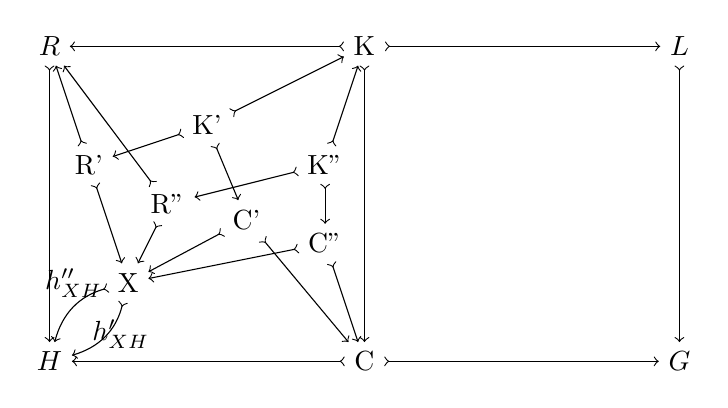
\begin{tikzpicture} 
            \node (k) at (0,0) {K};
            \node (c) at (0,-4) {C};
            \node (l) at (-4,0) {$R$};
            \node (g) at (-4,-4) {$H$};
            \node (r) at (4,0) {$L$};
            \node (h) at (4,-4) {$G$};
            \draw [>->] (k) -- (r); 
            \draw [>->] (c) -- (h);
            \draw [>->] (r) -- (h);
            \draw[>->] (l) -- (g) node [midway,above] {};
            \draw[>->] (c) -- (g) node [midway,above] {};
            \draw[>->] (k) -- (c) node[midway, left] {};
            \draw[<-<] (l) to (k);
            \node (k') at (-2,-1) {K'};
            \node (r') at (-3.5,-1.5) {R'};
            \node (c') at (-1.5,-2.2) {C'};
            \node (x) at (-3,-3) {X};
            \draw [>->] (c') -- (x);
            \draw [>->] (r') -- (x); 
            \draw [>->] (k') -- (r');
            \draw [>->] (k') -- (c');
            \draw [>->] (c') -- (c);
            \draw [>->] (r') -- (l);
            \draw [>->] (k') -- (k);

            \node (k'') at (-0.5,-1.5) {K''};
            \node (r'') at (-2.5,-2) {R''};
            \node (c'') at (-0.5,-2.5) {C''};
            \draw [>->] (c'') -- (x);
            \draw [>->] (r'') -- (x);
            \draw [>->] (k'') -- (r'');
            \draw [>->] (k'') -- (c'');
            \draw [>->] (k'') -- (k);
            \draw [>->] (c'') -- (c);
            \draw [>->] (r'') -- (l);

            \draw [>->] (x) edge[bend left] node[pos=0.1,below]{$h_{XH}'$} (g);
            \draw [>->] (x) edge[bend right] node[midway,above]{$h_{XH}''$} (g);

        \end{tikzpicture}
    \end{center}
    where $K'R'XC'$, $K''R''XC''$, $K'KCC'$, $K''KCC''$, $R'RHX$ and $R''RHX$ are pullbacks.

    By~\autoref{kpcpck_pullback}, $K'KLR'$ and $K''KCC''$ are pullbacks. 

    By~\autoref{kpcpxrp_po}, $K'R'XC'$ and $K''R''XC''$ are pushout.

    Since $\rho$ is $X$-non-increasing under $\Psi$, there are $\Psi(R'): R' \rightarrowtail L$ and $\Psi(R''):R'' \rightarrowtail L$ such that $K'R'LK$ and $K''R''LK$ are pullbacks.

    By~\autoref{lem:g_monic}, we have the following commutative diagram
    \begin{center}
        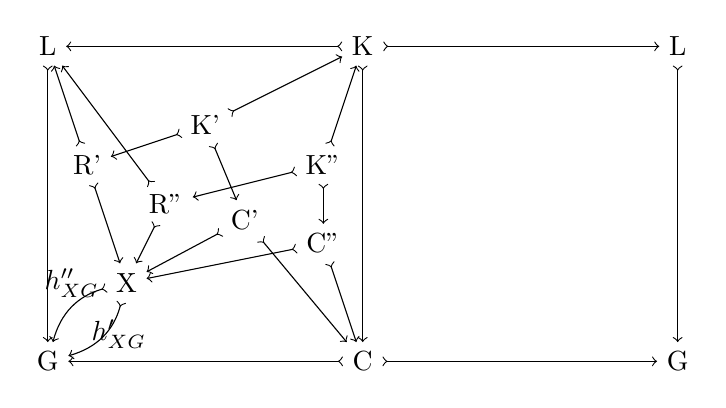
\begin{tikzpicture} 
            \node (k) at (0,0) {K};
            \node (c) at (0,-4) {C};
            \node (l) at (-4,0) {L};
            \node (g) at (-4,-4) {G};
            \node (r) at (4,0) {L};
            \node (h) at (4,-4) {G};
            \draw [>->] (k) -- (r); 
            \draw [>->] (c) -- (h);
            \draw [>->] (r) -- (h);
            \draw[>->] (l) -- (g) node [midway,above] {};
            \draw[>->] (c) -- (g) node [midway,above] {};
            \draw[>->] (k) -- (c) node[midway, left] {};
            \draw[<-<] (l) to (k);
            \node (k') at (-2,-1) {K'};
            \node (r') at (-3.5,-1.5) {R'};
            \node (c') at (-1.5,-2.2) {C'};
            \node (x) at (-3,-3) {X};
            \draw [>->] (c') -- (x);
            \draw [>->] (r') -- (x); 
            \draw [>->] (k') -- (r');
            \draw [>->] (k') -- (c');
            \draw [>->] (c') -- (c);
            \draw [>->] (r') -- (l);
            \draw [>->] (k') -- (k);

            \node (k'') at (-0.5,-1.5) {K''};
            \node (r'') at (-2.5,-2) {R''};
            \node (c'') at (-0.5,-2.5) {C''};
            \draw [>->] (c'') -- (x);
            \draw [>->] (r'') -- (x);
            \draw [>->] (k'') -- (r'');
            \draw [>->] (k'') -- (c'');
            \draw [>->] (k'') -- (k);
            \draw [>->] (c'') -- (c);
            \draw [>->] (r'') -- (l);

            \draw [>->] (x) edge[bend left] node[pos=0.1,below]{$h_{XG}'$} (g);
            \draw [>->] (x) edge[bend right] node[midway,above]{$h_{XG}''$} (g);

        \end{tikzpicture}
    \end{center}
    where  
    \begin{itemize}
        \item $K'R'XC'$ is pushout and pullback;
        \item $K''R''XC''$ is pushout and pullback;
        \item $K'KCC'$ and $K''KCC''$ are pullback;
        \item $h_{XG}':X \to G$ is the unique morphism such that $h_{C'C} \star h_{CG} = h_{C'X} \star h_{XG}'$ and  $h_{R'L} \star h_{LG} = h_{R'X} \star h_{XG}'$ where $h_{R'L} = \Psi(R')$;
        \item $h_{XG}'':X \to G$ is the unique morphism such that $h_{C''C} \star h_{CG} = h_{C''X} \star h_{XG}''$ and  $h_{R''L} \star h_{LG} = h_{R''X} \star h_{XG}''$ where $h_{R''L} = \Psi(R'')$.
    \end{itemize}
    If $h_{XH}' \neq h_{XH}''$ then $h_{XG}' \neq h_{XG}''$.
\end{lemma}
\begin{proof}
    Suppose that $h_{XH}' \neq h_{XH}''$. We are going to show $h_{XG}' \neq h_{XG}''$.

    From $h_{XH}' \neq h_{XH}''$, we deduce there exists an element $x \in X$ such that $h_{XH}(x) \neq h_{XH}''(x)$. We can suppose that \begin{flalign}
        \text{$x$ is either an isolated nodes or an edge.} \label{x_isolated_or_edge}
    \end{flalign}  \todo{$x$ is either an isolated node or an edge}
    because otherwise $x$ would be a non-isolated node and we can take an incident edge of $x$.

    \noindent
    Since $K'R'XC'$ and $K''R''XC''$ are pushouts, by~\autoref{lem:xinXcpinCrpinR}, there are 4 possible cases:
    \begin{enumerate}
        \item there are $c' \in C', c'' \in C''$ such that $h_{C'X}(c') = h_{C'X}(c'') = x$;
        \item  there are $r' \in R', r'' \in R''$ such that $h_{R'X}(r') = h_{R'X}(r'') = x$
        \item there are arrows $r' \in R'$ and $c'' \in C''$ such that 
        \begin{flalign*}
            h_{C''X}(c'') = x
            \\
            h_{R'X}(r') = x
            \\
            \nexists c' \in C'. h_{C'X}(c') = x 
            \\
            \nexists r'' \in R''. h_{R''X}(r'') = x 
        \end{flalign*}
        \item there are arrows $r'' \in R''$ and $c' \in C'$ such that 
        \begin{flalign*}
            h_{C'X}(c') = x
            \\
            h_{R''X}(r'') = x
            \\
            \nexists c'' \in C''. h_{C''X}(c'') = x 
            \\
            \nexists r' \in R'. h_{R'X}(r') = x   
        \end{flalign*}
    \end{enumerate}

    We are going to show that in each case we have $h_{XG}'(x) \neq h_{XG}''(x)$. Since the fourth case is symmetric to the third case, it suffices to analyse the first three cases.

    \begin{itemize}
        \item[(1)] Suppose that there are $c' \in C', c'' \in C''$ such that $h_{C'X}(c') = h_{C'X}(c'') = x$. 
        Suppose, by contradiction, that the following equality holds
        \begin{flalign}
            h_{C'C}(c') = h_{C''C}(c'') \label{cpccp_eq_cppccpp}
        \end{flalign}
         we have the following contradiction:
        \begin{flalign*}
            &h_{XH}'(x) \\
           =&h_{XH}'(h_{C'X}(c')) \\
           =&(h_{C'X} \star h_{XH}')(c') \\
           =&(h_{C'C} \star h_{CH})(c') &\text{By commutativity of $C'XHC$}\\
           =&h_{CH}(h_{C'C}(c')) \\
           =&h_{CH}(h_{C''C}(c'')) & \text{ by~\eqref{cpccp_eq_cppccpp}}\\
           =&(h_{C''C} \star h_{CH})(c'') \\
           =&(h_{C''X} \star h_{XH}'')(c'') &\text{By commutativity of $C''CHX$}\\
           =&h_{XH}''(h_{C''X}(c'')) \\
           = &h_{XH}''(x) \\
        \end{flalign*}
        
        % \begin{center}
        %     \begin{tikzpicture} 
        %         \node (k) at (0,0) {K};
        %         \node (c) at (0,-4) {C};
        %         \node (l) at (-4,0) {$L$};
        %         \node (g) at (-4,-4) {$G$};
        %         \draw[>->] (l) -- (g) node [midway,above] {};
        %         \draw[>->] (c) -- (g) node [midway,above] {};
        %         \draw[>->] (k) -- (c) node[midway, left] {};
        %         \draw[<-<] (l) to (k);
        %         \node (k') at (-2,-1) {K'};
        %         \node (r') at (-3.5,-1.5) {R'};
        %         \node (c') at (-1.5,-2.2) {C'};
        %         \node (x) at (-3,-3) {X};
        %         \draw [>->] (c') -- (x);
        %         \draw [>->] (r') -- (x); 
        %         \draw [>->] (k') -- (r');
        %         \draw [>->] (k') -- (c');
        %         \draw [>->] (c') -- (c);
        %         \draw [>->] (r') -- (l);
        %         \draw [>->] (k') -- (k);
    
        %         \node (k'') at (-0.5,-1.5) {K''};
        %         \node (r'') at (-2.5,-2) {R''};
        %         \node (c'') at (-0.5,-2.5) {C''};
        %         \draw [>->] (c'') -- (x);
        %         \draw [>->] (r'') -- (x);
        %         \draw [>->] (k'') -- (r'');
        %         \draw [>->] (k'') -- (c'');
        %         \draw [>->] (k'') -- (k);
        %         \draw [>->] (c'') -- (c);
        %         \draw [>->] (r'') -- (l);
    
        %         \draw [>->] (x) edge[bend left] node[pos=0.3,below]{!g''} (g);
        %         \draw [>->] (x) edge[bend right] node[midway,above]{!g'} (g);
    
        %     \end{tikzpicture}
        % \end{center}
        Therefore, we have 
        \begin{flalign}
            h_{C'C}(c') \neq h_{C''C}(c'') \label{cpccp_neq_cppccpp}
        \end{flalign} 
        \begin{flalign*}
            h_{XG}'(x)&= h_{XG}'(h_{C'X}(c')) & \text{by definition of $c'$}\\
                        &= (h_{C'X} \star h_{XG}')(c')  \\
                        &= (h_{C'C} \star h_{CG})(c') & \text{by commutativity of $C'CGX$} \\
                        &= h_{CG}(h_{C'C}(c')) &  \\
                        &\neq h_{CG}(h_{C''C}(c'')) & \text{by~\eqref{cpccp_neq_cppccpp} and the injectivity of $h_{CG}$} \\
                        &= (h_{C''C} \star h_{CG})(c'') &  \\
                        &= (h_{C''X} \star h_{XG}'')(c'') & \text{by commutativity of $C''CGX$} \\
                        &= h_{XG}''(h_{C''X}(c'')) \\
                        &= h_{XG}''(x) & \text{by definition of $c''$}
        \end{flalign*}
 
        \item[(2)] Suppose that there are $r' \in R', r'' \in R''$ such that $h_{R'X}(r') = h_{R'X}(r'') = x$. We have 
        \begin{flalign}
            h_{R'R}(r') \neq h_{R''R}(r'') \label{rprrppr}
        \end{flalign}  
        by an argument analogous to the argument for $h_{C'C}(c') \neq h_{C''C}(c'')$ in the previous case. Since $\rho$ is $X$-non-increasing,~\eqref{rprrppr} and~\eqref{x_isolated_or_edge} hold, we have \todo{use : x is either an isolated node or an edge}       
        \begin{flalign}
            h_{R'L}(r') \neq h_{R''L}(r'') \label{rplrprpplrpp}
        \end{flalign}  

        % Therefore, we have  
        % \begin{flalign*}
        %     h_{XG}'(x)&= h_{XG}'(h_{R'X}(r')) & \text{by definition of $r'$}\\
        %         &= (h_{R'X} \star h_{XG}')(r')  \\
        %         &= (h_{R'L} \star h_{LG})(r') & \text{by commutativity of $R'LGX$} \\
        %         &= h_{LG}(h_{R'L}(r')) &  \\
        %         &\neq h_{LG}(h_{R''L}(r'')) & \text{by $h_{R'R}(r') \neq h_{R''R}(r'')$ and the injectivity of $h_{RG}$} \\
        %         &= (h_{R''L} \star h_{LG})(r'') &  \\
        %         &= (h_{R''X} \star h_{XG}'')(r'') & \text{by commutativity of $R''LGX$} \\
        %         &= h_{XG}''(h_{R''X}(r'')) \\
        %         &= h_{XG}''(x) & \text{by definition of $r''$}
        % \end{flalign*}
         
        % \todo{$h_{R_XL}$ edge-injective} Since $h_{R_XL}$ is edge-injective by assumption, because it is $X$-non-increasing by assumption. Therefore, we have $h_{R'L}(r') \neq h_{R''L}(r'')$ because \( h_{R'R}(r') \neq h_{R''R}(r'') \). Hence, from~\ref{rprneqrppr}, we have 
        % \begin{flalign}
        %     h_{R'L}(r') \neq h_{R''L}(r'') \label{rplrprpplrpp}
        % \end{flalign}
        Hence, the following inequality holds
        
        % \begin{center}
        %     \begin{tikzpicture} 
        %         \node (k) at (0,0) {K};
        %         \node (c) at (0,-4) {C};
        %         \node (l) at (-4,0) {$L$};
        %         \node (g) at (-4,-4) {$G$};
        %         \draw[>->] (l) -- (g) node [midway,above] {};
        %         \draw[>->] (c) -- (g) node [midway,above] {};
        %         \draw[>->] (k) -- (c) node[midway, left] {};
        %         \draw[<-<] (l) to (k);
        %         \node (k') at (-2,-1) {K'};
        %         \node (r') at (-3.5,-1.5) {R'};
        %         \node (c') at (-1.5,-2.2) {C'};
        %         \node (x) at (-3,-3) {X};
        %         \draw [>->] (c') -- (x);
        %         \draw [>->] (r') -- (x); 
        %         \draw [>->] (k') -- (r');
        %         \draw [>->] (k') -- (c');
        %         \draw [>->] (c') -- (c);
        %         \draw [>->] (r') -- (l);
        %         \draw [>->] (k') -- (k);
    
        %         \node (k'') at (-0.5,-1.5) {K''};
        %         \node (r'') at (-2.5,-2) {R''};
        %         \node (c'') at (-0.5,-2.5) {C''};
        %         \draw [>->] (c'') -- (x);
        %         \draw [>->] (r'') -- (x);
        %         \draw [>->] (k'') -- (r'');
        %         \draw [>->] (k'') -- (c'');
        %         \draw [>->] (k'') -- (k);
        %         \draw [>->] (c'') -- (c);
        %         \draw [>->] (r'') -- (l);
    
        %         \draw [>->] (x) edge[bend left] node[pos=0.3,below]{!g''} (g);
        %         \draw [>->] (x) edge[bend right] node[midway,above]{!g'} (g);
    
        %     \end{tikzpicture}
        % \end{center}
        \begin{flalign*}
            h_{XG}'(x) &= h_{XG}'(h_{R'X}(r')) & \text{by definition of $r'$}\\
                         &= (h_{R'X} \star h_{XG}')(r')  \\
                         &= (h_{R'L} \star h_{LG})(r') & \text{by commutativity of $R'XGL$} \\
                         &= h_{LG}(h_{R'L}(r')) &  \\
                         &\neq h_{LG}(h_{R''L}(r'')) &  \text{By injectivity of $h_{LG}$ and~\eqref{rplrprpplrpp}}\\
                         &= (h_{R''L} \star h_{LG})(r'') &  \\
                         &= (h_{R''X} \star h_{XG}'')(r'') & \text{by commutativity of $R''XGL$} \\
                         &= h_{XG}''(h_{R''X}(r'')) \\
                         &= h_{XG}''(x) & \text{by definition of $r''$}
        \end{flalign*}  
        
        % \begin{center}
        %     \begin{tikzpicture} 
        %         \node (k) at (0,0) {K};
        %         \node (c) at (0,-4) {C};
        %         \node (l) at (-4,0) {$L$};
        %         \node (g) at (-4,-4) {$G$};
        %         \draw[>->] (l) -- (g) node [midway,above] {};
        %         \draw[>->] (c) -- (g) node [midway,above] {};
        %         \draw[>->] (k) -- (c) node[midway, left] {};
        %         \draw[<-<] (l) to (k);
        %         \node (k') at (-2,-1) {K'};
        %         \node (r') at (-3.5,-1.5) {R'};
        %         \node (c') at (-1.5,-2.2) {C'};
        %         \node (x) at (-3,-3) {X};
        %         \draw [>->] (c') -- (x);
        %         \draw [>->] (r') -- (x); 
        %         \draw [>->] (k') -- (r');
        %         \draw [>->] (k') -- (c');
        %         \draw [>->] (c') -- (c);
        %         \draw [>->] (r') -- (l);
        %         \draw [>->] (k') -- (k);
    
        %         \node (k'') at (-0.5,-1.5) {K''};
        %         \node (r'') at (-2.5,-2) {R''};
        %         \node (c'') at (-0.5,-2.5) {C''};
        %         \draw [>->] (c'') -- (x);
        %         \draw [>->] (r'') -- (x);
        %         \draw [>->] (k'') -- (r'');
        %         \draw [>->] (k'') -- (c'');
        %         \draw [>->] (k'') -- (k);
        %         \draw [>->] (c'') -- (c);
        %         \draw [>->] (r'') -- (l);
    
        %         \draw [>->] (x) edge[bend left] node[pos=0.3,below]{!g''} (g);
        %         \draw [>->] (x) edge[bend right] node[midway,above]{!g'} (g);
    
        %     \end{tikzpicture}
        % \end{center}
        \item[(3)] Suppose, that there are arrows $r' \in R'$ and $c'' \in C''$ such that 
        \begin{flalign*}
            h_{C''X}(c'') = x
            \\
            h_{R'X}(r') = x
            \\
            \nexists c' \in C'. h_{C'X}(c') = x 
        \end{flalign*}
        \begin{flalign}
            \nexists r'' \in R''. h_{R''X}(r'') = x  \label{assumption_norpp}
        \end{flalign}

        Suppose, by contradiction, that we have \begin{flalign}
            h_{C''C}(c'') \in \operatorname{Im}(h_{KC})  \label{assump_c_in_imhkc}
        \end{flalign} 
        Then,
        there are $k_2 \in K$ such that $h_{KC}(k_2) = h_{C''C}(c'')$.

        There is $k'' \in K''$ such that $h_{K''K}(k'') = k_2$ and $h_{K''C''}(k'') = c''$ becase $K''C''CK$ is a pullback square and $h_{KC}(k_2) = h_{C''C}(c'')$.

        We have $h_{K''R''}(k'') \in R''$ and 
        \begin{flalign*}
          &h_{R''X}(h_{K''R''}(k''))\\
         =&(h_{K''R''} \star h_{R''X})(k'') \\
         =&(h_{K''C''} \star h_{C''X})(k'') & \text{by commutativity of $K''R''XC''$}\\
         =&h_{C''X}(h_{K''C''}(k''))\\
         =&h_{C''X}(c'')\\
         =&x
        \end{flalign*}
        which contradicts the assumption~\eqref{assumption_norpp}.
        
        Thus, the following holds
        \begin{flalign}
            h_{C''C}(c'') \notin \operatorname{Im}(h_{KC})  \label{assump_c_notin_imhkc}
        \end{flalign} 

        We deduce
        \begin{flalign*}
            h_{XG}'(x) &= h_{XG}'(h_{C''X}(c'')) & \text{by definition of $c''$}\\
                         &= (h_{C''X} \star h_{XG}')(c'') \\
                         &= (h_{C''C} \star h_{CG})(c'') & \text{by commutativity of $C''CGX$} \\
                         &= h_{CG}(h_{C''C}(c'')) &  \\
                         &\neq  h_{LG}(h_{R'L}(r')) & \text{by~\autoref{lem:b_c_same_img_exist_a} and the assumption~\eqref{assump_c_notin_imhkc}} \\
                         &= (h_{R'L} \star h_{LG})(r') \\
                         &= (h_{R'X} \star h_{XG}'')(r') & \text{by commutativity of $R'XGL$} \\
                         &= h_{XG}''(h_{R'X}(r'))\\
                         &= h_{XG}''(x) & \text{by definition of $r'$}
        \end{flalign*} 

    %     We analyse the two cases where $h_{C''C}(c'') \notin \operatorname{Im}(h_{KC}) $ and 
    %         \begin{itemize}
    %             \item[(3.1)] Suppose, that the following holds
    %                 \begin{flalign}
    %                     h_{C''C}(c'') \notin \operatorname{Im}(h_{KC})  \label{assump_c_notin_imhkc}
    %                 \end{flalign} then, we have 
    %                 \begin{flalign*}
    %                     h_{XG}'(x) &= h_{XG}'(h_{C''X}(c'')) & \text{by definition of $c''$}\\
    %                                  &= (h_{C''X} \star h_{XG}')(c'') \\
    %                                  &= (h_{C''C} \star h_{CG})(c'') & \text{by commutativity of $C''CGX$} \\
    %                                  &= h_{CG}(h_{C''C}(c'')) &  \\
    %                                  &\neq  h_{LG}(h_{R'L}(r')) & \text{by~\autoref{lem:b_c_same_img_exist_a} and the assumption~\eqref{assump_c_notin_imhkc}} \\
    %                                  &= (h_{R'L} \star h_{LG})(r') \\
    %                                  &= (h_{R'X} \star h_{XG}'')(r') & \text{by commutativity of $R'XGL$} \\
    %                                  &= h_{XG}''(h_{R'X}(r'))\\
    %                                  &= h_{XG}''(x) & \text{by definition of $r'$}
    %                 \end{flalign*} 
    %             \item[(3.2)] Suppose, that the following holds
    %             \begin{flalign}
    %                 h_{R'R}(r') \notin \operatorname{Im}(h_{KR}) \label{rprrp_im_kr}
    %             \end{flalign} 
    %             Since $\rho$ is $X$-non-increasing, by the assumption~\eqref{rprrp_im_kr}, (\autoref{def:creates_more_x_on_the_left})$h_{R'L}$ does not identify non-interface elements with interface elements. Therefore, the following holds 
    %             \begin{flalign}
    %                 h_{R'L}(r') \notin \operatorname{Im}(h_{KL}) \label{lnotinhkl}
    %             \end{flalign} 
    %             \todo{assumption: does not identify non-interface elements with interface elements} 
    %             Therefore, 
    %     
    %     % \begin{center}
    %     %     \begin{tikzpicture} 
    %     %         \node (k) at (0,0) {K};
    %     %         \node (c) at (0,-4) {C};
    %     %         \node (l) at (-4,0) {$L$};
    %     %         \node (g) at (-4,-4) {$G$};
    %     %         \draw[>->] (l) -- (g) node [midway,above] {};
    %     %         \draw[>->] (c) -- (g) node [midway,above] {};
    %     %         \draw[>->] (k) -- (c) node[midway, left] {};
    %     %         \draw[<-<] (l) to (k);
    %     %         \node (k') at (-2,-1) {K'};
    %     %         \node (r') at (-3.5,-1.5) {R'};
    %     %         \node (c') at (-1.5,-2.2) {C'};
    %     %         \node (x) at (-3,-3) {X};
    %     %         \draw [>->] (c') -- (x);
    %     %         \draw [>->] (r') -- (x); 
    %     %         \draw [>->] (k') -- (r');
    %     %         \draw [>->] (k') -- (c');
    %     %         \draw [>->] (c') -- (c);
    %     %         \draw [>->] (r') -- (l);
    %     %         \draw [>->] (k') -- (k);
    
    %     %         \node (k'') at (-0.5,-1.5) {K''};
    %     %         \node (r'') at (-2.5,-2) {R''};
    %     %         \node (c'') at (-0.5,-2.5) {C''};
    %     %         \draw [>->] (c'') -- (x);
    %     %         \draw [>->] (r'') -- (x);
    %     %         \draw [>->] (k'') -- (r'');
    %     %         \draw [>->] (k'') -- (c'');
    %     %         \draw [>->] (k'') -- (k);
    %     %         \draw [>->] (c'') -- (c);
    %     %         \draw [>->] (r'') -- (l);
    
    %     %         \draw [>->] (x) edge[bend left] node[pos=0.3,below]{!g''} (g);
    %     %         \draw [>->] (x) edge[bend right] node[midway,above]{!g'} (g);
    
    %     %     \end{tikzpicture}
    %     % \end{center}
    %                 \begin{flalign*}
    %                     h_{XG}'(x) &= h_{XG}'(h_{R'X}(r')) & \text{by definition of $r'$}\\
    %                                  &= (h_{R'X} \star h_{XG}')(r') \\
    %                                  &= (h_{R'L} \star h_{LG})(r') & \text{by commutativity of $R'LGX$} \\
    %                                  &= h_{LG}(h_{R'L}(r')) &  \\
    %                                  &= h_{CG}(h_{C''C}(c'')) & \text{by~\autoref{lem:b_c_same_img_exist_a} and the assumption~\eqref{lnotinhkl}}  \\
    %                                  &= (h_{C''C} \star h_{CG})(c'') \\
    %                                  &= (h_{C''X} \star h_{XG}'')(c'') & \text{by commutativity of $C''XGC$} \\
    %                                  &= h_{XG}''(h_{C''X}(c''))\\
    %                                  &= h_{XG}''(x) & \text{by definition of $c''$}
    %                 \end{flalign*}
    %                  \newpage  
    %          
    % \begin{center}
    %         \begin{tikzpicture} 
    %             \node (k) at (0,0) {K};
    %             \node (c) at (0,-4) {C};
    %             \node (l) at (-4,0) {$L$};
    %             \node (g) at (-4,-4) {$G$};
    %             \draw[>->] (l) -- (g) node [midway,above] {};
    %             \draw[>->] (c) -- (g) node [midway,above] {};
    %             \draw[>->] (k) -- (c) node[midway, left] {};
    %             \draw[<-<] (l) to (k);
    %             \node (k') at (-2,-1) {K'};
    %             \node (r') at (-3.5,-1.5) {R'};
    %             \node (c') at (-1.5,-2.2) {C'};
    %             \node (x) at (-3,-3) {X};
    %             \draw [>->] (c') -- (x);
    %             \draw [>->] (r') -- (x); 
    %             \draw [>->] (k') -- (r');
    %             \draw [>->] (k') -- (c');
    %             \draw [>->] (c') -- (c);
    %             \draw [>->] (r') -- (l);
    %             \draw [>->] (k') -- (k);
    
    %             \node (k'') at (-0.5,-1.5) {K''};
    %             \node (r'') at (-2.5,-2) {R''};
    %             \node (c'') at (-0.5,-2.5) {C''};
    %             \draw [>->] (c'') -- (x);
    %             \draw [>->] (r'') -- (x);
    %             \draw [>->] (k'') -- (r'');
    %             \draw [>->] (k'') -- (c'');
    %             \draw [>->] (k'') -- (k);
    %             \draw [>->] (c'') -- (c);
    %             \draw [>->] (r'') -- (l);
     
    %             \draw [>->] (x) edge[bend left] node[pos=0.3,below]{!g''} (g);
    %             \draw [>->] (x) edge[bend right] node[midway,above]{!g'} (g);
    
    %         \end{tikzpicture}
    %     \end{center}

    %             \item[(3.3)]  
    %             Suppose, 
    %             \color{red}
    %             that \begin{flalign}
    %                 h_{R'R}(r') \in h_{KR}(K) 
    %                 \\
    %                 h_{C''C}(c'') \in h_{KC}(K)
    %             \end{flalign}
    %             Thus,
    %             there are $k_1, k_2 \in K$ such that $h_{KR}(k_1) = h_{R'R}(r')$ and $h_{KC}(k_2) = h_{C''C}(c'')$.
    %             \color{black}

    %             There is $k'' \in K''$ such that $h_{K''K}(k'') = k_2$ and $h_{K''C''}(k'') = c''$ becase $K''C''CK$ is a pullback square and $h_{KC}(k_2) = c = h_{C''C}(c'')$.

    %             We cannot have $k_1=k_2$. Suppose, by contradiction, that we have $k_1=k_2$. 
    %             \color{red} 
    %             Let $r'' = h_{K''R''}(k'')$. We have 
    %             \begin{flalign}
    %                 &h_{R''R}(r'')\\
    %                =&h_{R''R}(h_{K''R''}(k''))\\
    %                =&(h_{K''R''} \star h_{R''R})(k'') & \text{by definition of $r''$}\\
    %                =&(h_{K''K} \star h_{KR})(k'') &\text{by commutativity of $K''R''RK$}\\
    %                =&h_{KR}(h_{K''K}(k''))  \\
    %                =&h_{KR}(k_1) & \text{by definition of $k_1$} \\
    %                =&r
    %             \end{flalign}
    %             \color{black}
    %             % We have therefore $h_{K''C''}(k'') = c''$ because $h_{C''C}$ is injective, $h_{C''C}(c'') = c$ and 
    %             % \begin{flalign*}
    %             %    &h_{C''C}(h_{K''C''}(k'')) \\
    %             %   =&(h_{K''C''} \star h_{C''C})(k'')\\
    %             %   =&(h_{K''K} \star h_{KC})(k'')\\
    %             %   =&h_{KC}(h_{K''K}(k''))\\
    %             %   =&h_{KC}(k_2)\\
    %             %   =&c
    %             % \end{flalign*}
    %             and 
    %             \begin{flalign*}
    %               &h_{R''X}(r'')\\
    %              =&h_{R''X}(h_{K''R''}(k'')) \\
    %              =&(h_{K''R''} \star h_{R''X})(k'') \\
    %              =&(h_{K''C''} \star h_{C''X})(k'') & \text{by commutativity of $K''R''XC''$}\\
    %              =&h_{C''X}(h_{K''C''}(k''))\\
    %              =&h_{C''X}(c'')\\
    %              =&x
    %             \end{flalign*}


    %             \begin{flalign*}
    %                =&h_{R''X}(h_{K''R''}(k'')) \\
    %                =&(h_{K''R''} \star h_{R''X})(k'') \\
    %                =&(h_{K''C''} \star h_{C''X})(k'') & \text{by commutativity of $K''R''XC''$}\\
    %                =&h_{C''X}(h_{K''C''}(k''))\\
    %                =&h_{C''X}(c'')\\
    %                =&x
    %               \end{flalign*}

    %                     \begin{flalign*}
    %                         x &= h_{C''X}(c'')  & \text{by definition of $r''$}\\
    %                             &= h_{C''X}(h_{K'C''}(k')) & \text{by definition of $k'$}\\
    %                             &= (h_{K'C''} \star h_{C''X})(k') &  \\
    %                             &= (h_{K'R'} \star h_{R'X})(k') & \text{by the commutativity of $K'C'XR'$} \\
    %                             &= h_{R'X}(h_{K'R'}(k')) &  \\
    %                             &= h_{R'X}(r') &  \text{by definition of $k'$}\\
    %                             &= x& \text{by definition of $r'$}
    %                     \end{flalign*}
    %             which contradic the assumption~\eqref{assumption_norpp}.

    %             Hence \begin{flalign}
    %                 k_1 \neq k_2 \label{k1_neq_k2}
    %             \end{flalign}

    %             From~\eqref{k1_neq_k2}, we have 
    %             \begin{flalign}
    %                 h_{KR}(k_1) \neq h_{KR}(k_2) \label{hkrk1_neq_hkrk2}
    %             \end{flalign} 

    %             Since~\eqref{hkrk1_neq_hkrk2} holds and $\rho$ is $X$-non-increasing, we have 
    %             \begin{flalign}
    %                 h_{KL}(k_1) \neq h_{KR}(k_2) \label{hkrk1_neq_hkrk2}
    %             \end{flalign} 

    %             By assumption on $\rho$ \todo{assumption: non-increasing}, we have $h_{KL}(k_2) = h_{R'L}(r') = l$ for some $k_2 \in K$.
                
    %             \begin{flalign*}
    %                 h_{XG}(x) &= h_{XG}(h_{C''X}(c'')) & \text{by definition of $c''$} \\
    %                         &= (h_{C''X} \star h_{XG})(c') &  \\
    %                         &= (h_{C''C} \star h_{CG})(c'') & \text{by commutativity of $C''CGX$} \\
    %                         &= h_{CG}(h_{C''C}(c'')) &  \\
    %                         &= h_{CG}(c) & \text{by definition of $c$} \\
    %                         &= h_{CG}(h_{KC}(k_1)) & \text{by definition of $k_1$} 
    %                         \\
    %                         &= (h_{KC} \star h_{CG})(k_1) & 
    %                         \\
    %                         &\neq (h_{KC} \star h_{CG})(k_2) & \text{by~\eqref{k1_neq_k2} and injectivity of $h_{KC} \star h_{CG}$} 
    %                         \\
    %                         &= (h_{KL} \star h_{LG})(k_2) & 
    %                         \\
    %                         &= h_{LG}(h_{KL}(k_2)) & 
    %                         \\
    %                         &= h_{LG}(h_{R'L}(r')) & 
    %                         \\
    %                         &= (h_{R'L} \star h_{LG})(r') & 
    %                         \\
    %                         &= (h_{R'X} \star h_{XG})(r') & \text{by commutativity of $R'LGX$} \\
    %                         &= h_{XG}(h_{R'X}(r'))\\
    %                             &= h_{XG}(x) & \text{by definition of $r'$}
    %             \end{flalign*}
              
    %         \end{itemize}            
    \end{itemize}
\end{proof}